\usetikzlibrary{arrows.meta}
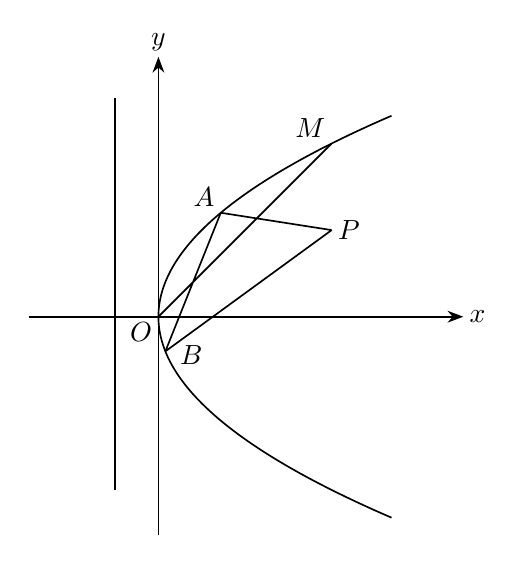
\begin{tikzpicture}[x=2.2cm,y=2.2cm,line width=.6pt,>=Stealth,font=\normalsize]
\coordinate (O) at (0,0);
\coordinate (M) at (1,1);
\coordinate (P) at (1,0.5);
\coordinate (A) at (0.36,0.6);
\coordinate (B) at (0.04,-0.2);
\draw[->] (-0.75,0)--(1.76,0) node[right,inner sep=2pt] {$x$};
\draw[->] (0,-1.26)--(0,1.5) node[above,inner sep=2pt] {$y$};
\draw (-0.25,-1.0)--(-0.25,1.26);
\draw plot[domain=-1.16:1.16,samples=121] (\x*\x,\x);
\draw (O)--(M) (A)--(B) (A)--(P) (B)--(P);
\node[below left,inner sep=2pt] at (O) {$O$};
\node[above left,inner sep=2pt] at (M) {$M$};
\node[right,inner sep=2pt] at (P) {$P$};
\node[above left,inner sep=2pt] at (A) {$A$};
\node at (0.19,-0.22) {$B$};
\end{tikzpicture}
